\documentclass[8pt, landscape, fleqn]{scrartcl}
\setlength{\parindent}{0pt}
\usepackage[ngerman]{babel}
%\usepackage[applemac]{inputenc}
\usepackage[utf8]{inputenc}
\usepackage[dvips]{geometry}
\usepackage{latexsym}
\usepackage{multicol}
\usepackage{amsmath}
\usepackage{graphicx}
\usepackage{array}
\usepackage{booktabs}
\usepackage{amsmath}
\usepackage{mathtools}
\usepackage{ulem}
\usepackage{amsfonts}
\usepackage{dsfont}
\usepackage{charter} %%% Schreibart
%\renewcommand{\familydefault}{\sfdefault}



%%%%%%%%%%Paket für Chemische Formeln
\usepackage{chemformula} 
\usepackage[version=3]{mhchem}
%%%%%%%%%%%%%%%%% Farbe
\usepackage{color}

\pagestyle{plain}
\typearea{20}
\columnsep 30pt
\columnseprule .4pt
\setlength{\extrarowheight}{0.9em}

\renewcommand{\arraystretch}{0.8}

\makeatletter
\renewcommand{\section}{\@startsection{section}{1}{0mm}%
{-2\baselineskip}{0.8\baselineskip}%
{\hrule depth 0.2pt width\columnwidth\hrule depth1.5pt
width0.25\columnwidth\vspace*{1.2em}\Large\bfseries\rmfamily}}
\makeatother


\makeatletter
\renewcommand{\subsection}{\@startsection{subsection}{1}{0mm}%
{-2\baselineskip}{0.8\baselineskip}%
{\hrule depth 0.2pt width\columnwidth\hrule depth0.75pt
width0.25\columnwidth\vspace*{1.2em}\large\bfseries\rmfamily}}
\makeatother

\makeatletter
\renewcommand{\subsubsection}{\@startsection{subsubsection}{1}{0mm}%
{-2\baselineskip}{0.8\baselineskip}%
{\hrule depth 0.2pt width\columnwidth\vspace*{1.2em}\normalsize\bfseries\rmfamily}}
\makeatother

\newcommand{\Mx}[1]{\begin{bmatrix}#1\end{bmatrix}}
\begin{document}
\part*{\LARGE\textrm{Ökonomie $\hfill$ Xeno Meienberg}}
\begin{multicols*}{3}

\section{Einführung}

\subsection{Gegenstand der Ökonomie}

\begin{itemize}
    \item Mikroökonomie (2,3,5,6,7)
    \item Makroökonomie (8-11)
\end{itemize}

Die Mikroökonomie befasst sich mit wirtschaftlichen Entscheidungen der einzelnen Haushalte und Unternehmen:

\begin{itemize}
    \item Nachfrage (nach Gütern, Arbeit)
    \item Angebot (an Gütern, Arbeit)
    \item Marktgeschehen (Markformen, Marktpreise, Gleichgewichte)
\end{itemize}

Die Makroökonomie befasst sich mit gesamtwirtschaftlichen Zusammenhängen

\begin{itemize}
    \item Aussenwirtschaftstheorie und -politik 
    \item Geldtheorie und -politik 
    \item Arbeitsmarkttheorie und -politik 
\end{itemize}

Die Rolle der Ökonomie: 

\begin{itemize}
    \item Ökonomie ist eine Denkmethode
    \item ...ist eine Sozialwissenschaft
    \item ...keine eindeutige Wissenschaft
    \item beantwortet die Fragen:
    \item Warum Menschen könomische Entscheidungen treffen
    \item ...wie man aus knappen Ressourcen das Optimum herausholen kann
    \item ...dass Ziele möglichst gut erreicht werden 
    \item ...Ökonomisches Denken bedeutet die Warhnehmung von Zielkonflikten und das Auswählen von Alternativen
    \item ...Differenz zwischen Ertrag und Kosten maximiert wird
\end{itemize}

\subsection{Methodisches Vorgehen der Ökonomie}

\begin{enumerate}
    \item Feststelung eines Problems
    \item Analyse, Theorie, Modelle (Annahmen, Abstraktion, Empirische Tests)
    \item Politik (Handlungsempfehlungen)
\end{enumerate}

\subsection{Gesellschaftliche Bedeutung ökonomischer Analysen}

Grundidee: Knappe Ressourcen optimal einsetzen für grössten Nutzen (Wohlfahrt) Ressourcen sind:

\begin{itemize}
    \item Natürliche Ressourcen
    \item Human Ressources 
    \item Sachliche Ressourcen / Sachkapital
    \item Soziale Ressourcen / Spielregeln 
\end{itemize}

Eine der Hauptfragen der Ökonomie: Gegeben Potential (Ressoucenportfolio), was ist das Maxmimum an Wohlfahrt dass man erreichen kann? Die Kernfragen zu beantworten sind: 

\begin{enumerate}
    \item Was soll produziert werden?
    \item Wie sollen Güter und Dienstleistungen produziert werden?
    \item Wie und an wen sollen die produzierten Güter und Dienstleistungen verteilt werden? Wer konsumiert?
\end{enumerate}

\textbf{Transformationskuve}: Menge zweier Güter $X_1$ und $X_2$ (Outputs), die in einer Gesellschaft maximal bei gegebenen Ressourcen produziert werden können. \newline \newline
\textbf{Produktions-Effizienz}: Ein Güterbündel ist produktionseffizient, wenn es zu den minimal möglichen Kosten hergestellt wird oder wenn es zu gegebenen Kosten kein anderes Güterbündel gibt, für welches eines der beiden Güter grösser ist als möglich. Ein produktionseffizientes Güterbündel liegt auf der Transformationskuve. \newline \newline 
\textbf{Opportunitätskosten}: Ressultiert aus der Tatsache, dass Ressourcen knapp sind. Die Mehrproduktion eines Guts führt zu einer kleineren Menge eines anderen Guts. Die Minderproduktion werden Opportunitätskosten genannt. \newline \newline
\textbf{Indifferenzkurven}: Die Kurve stellt alle Outputkombinationen dar, zwischen denen die Gesellschaft (oder Individuum) indifferent ist. Je weiter die Indifferenzkurven vom Ursprung entfernt sind, umso höher ist der Nutzen (das Niveau) der jeweiligen Kurve \newline \newline
\textbf{Wohlfahrtsmaximum}: Ist der Punkt wo die Menge des Gutes 1 und 2 produziert werden müssen damit die Gesellschaft ihr Wohlfahrtsmaximum erreichen wird. (Muss auf der Transformationskuve sein) \newline \newline
\textbf{Allokations-Effizienz / Pareto-Optimal}: Eine Verteilung ist pareto-optimal, wenn keine Verteilung möglich ist, welche von mindestens einem Individuum bevorzugt wird, jedoch niemand anderes benachteiligt.  
\section{Haushalte und Nachfrage}

\subsection{Grundlegende Annahmen für Nachfrage- und Angebotsverhalten}

\textbf{Annahmen}
\begin{itemize}
    \item Raum: Keine Entfernungen vorhanden 
    \item Zeit: Zeit spielt keine Rolle 
    \item Güter: Güter sind homogen (Keine Qualitätsunterschiede zwischen Produkten)
    \item Personen: Es gibt keine Vorlieben oder Abneigungen (alle gleich)
    \item Informtationen: Es herrscht vollständige Informtationen (alle informiert über Markt für Entscheidungen)
\end{itemize}

\textbf{Ökonomische Entscheidungen} für private Haushalte 

\begin{itemize}
    \item Nachfrage von Gütern und Dienstleistungen
    \item Angebot von Ressourcen (Arbeit und Kapital)
    \item Konsum heute vs. morgen 
\end{itemize}

\subsection{Marktnachfrage nach Gütern und Dienstleistungen}

\textbf{Nachfrage}: $x^N$ ist eine Funktion des Preises $p$ eines Gutes. Üblicherweise sinkt die Nachfrage mit steigendem Preis. Grund hierfür sind empirisch oder durch Maximierung des Nutzens und Nebenbedingung der Budgetrestriktion 

\begin{center}
    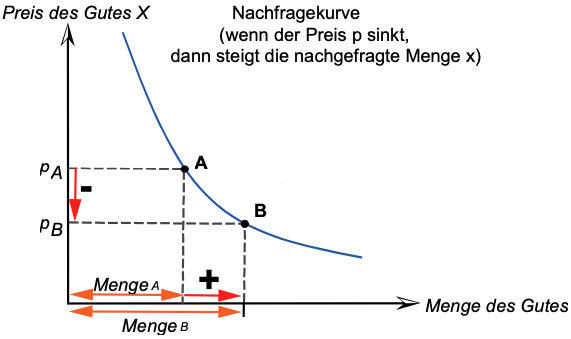
\includegraphics[width=7cm]{Typische_Nachfragefunktion.png}
\end{center}

\subsection{Ein Modell zu Konsumentscheidungen von Haushalten}

\subsubsection{Budgetrestriktion}

\textbf{Budgetrestriktion}: Summe der Ausgaben für zwei verschiedene Güter ($x_1p_1 + x_2p_2$) entsrpicht einem Budget $B$

\begin{align}
    B = x_1p_1 + x_2p_2 \\
    x_2 = \frac{B}{p_2} - x_1 \frac{p_1}{p_2}
\end{align}

Wie bereits erwähnt, ist der Nutzen eine lineare Kombination von preisen und Menge an Gütern, welche für eine Indifferenzkurve auf dem gleichen Niveau liegt die Gruppe oder Schar der Niveaulienen ergeben ein Nutzengebirge

\begin{equation}
    U = C x_1^a x_2^b
\end{equation}

mit $C$, $a$, $b$ Konstanten ($a,b =$ Bedeutung des Guts)

\subsubsection{Indifferenzkurven}

\textbf{Der Grenznutzen}: Ist die Ableitung einer Indifferenzkurve auf dem Niveau $U$ bezüglich $x_1$ und $x_2$ und ist immer positiv: 

\begin{equation}
    \frac{\partial U}{\partial x_1}, \frac{\partial U}{\partial x_2} > 0
\end{equation}

\textbf{Der Grenznutzen nimmt ab}. Der Nutzenzuwachs nimmt immer mehr ab mit zunehmenden Gütern einer Sorte (Es gitb eine Sättigung):

\begin{equation}
    \frac{\partial^2 U}{\partial x_1^2}, \frac{\partial^2 U}{\partial x_2^2} < 0
\end{equation}

Die Grenzrate der Substitution (GRS) misst die substituierbarkeit zweier Produkte und bestimmen die Form der Indifferenzkurve: 

\begin{equation}
   GRS =  \frac{GN_2}{GN_1} = \frac{dU/dx_2}{dU/dx_1}
\end{equation}

wobei perfekte Substitute bei $GRS = 1$ und perfekte Komplement bei $GRS = \pm \infty, 0$ 

\subsubsection{Der optimale Konsumpunkt}

\textbf{Der optimale Konsumpunkt}: Ist derjenige Punkt, wo sich Budgetrestriktion und Indifferenzkurve sich tangieren. Es ist dabei der maximale Nutzen bei gegebenem Budget. Die Steigung lautet hier $GRS$ bzw. $p_1/p_2$. Preisverhältnis = Grenzrate der Substitution/Grenznutzenverhältnis

\subsection{Von der optimalen Entscheidung zur individuellen Nachfragefunktion}

\begin{enumerate}
    \item Preis nimmt zu $\rightarrow$ Budgetrestriktion dreht sich 
    \item Es ergibt sich ein neues Nutzenniveau mit neuem Optimum
    \item Die nachgefragte Menge nimmt ab 
\end{enumerate}

Die Nachfragekurve zeigt die Zahlungsbereitschaft des Kosnumenten und kann auch als Funktion des Grenznutzens in Abhängigkeit von der Gütermenge interpretiert werden. Damit wird Nutzen und der marginale Nutzenzuwachs quantifizierbar und daher vergleichbar. 
Falls das Budget des Konsumenten sich ändert, oder seine Präferenzen sich änderen, kann verschiebt sich die Nachfragekurve nach oben oder nach unten. 

\begin{center}
    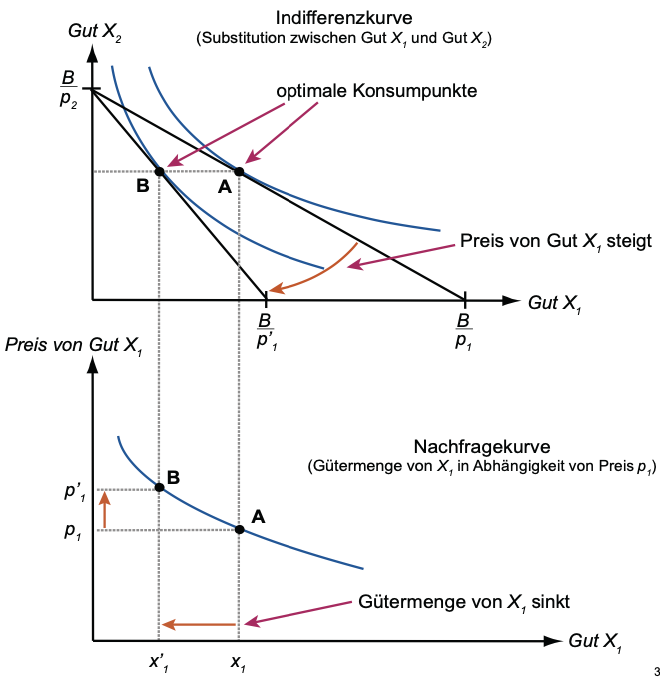
\includegraphics[width=7cm]{Nachfragefunktion.png}
\end{center}

\subsection{Preiselastizität der Nachfrage}

Die Preiselastizität der Nachfrage gibt an, um wie viel Prozent sich die nachgefragte Menge eines Gutes sich ändert als Folge einer einprozentigen Veränderung
des Preises dieses Gutes:

\begin{equation}
    \varepsilon_x N_p = \frac{\text{relative Mengenänderung}}{\text{relative Preisänderung}} = \frac{\frac{\Delta x^N}{x^N}}{\frac{\Delta p}{p}} = \frac{\Delta x^N}{\Delta p}\frac{p}{x^N}
\end{equation}

Im Grenzübergang $\Delta \rightarrow \partial$ beziehungsweise $\Delta p \rightarrow 0$:

\begin{equation}
    \varepsilon_x N_p = \frac{\partial x}{\partial p}\frac{p}{x^N}
\end{equation}

Die Preiselastizität hängt also von der Steigung der Nachfragekurve ($\frac{\partial x}{\partial p}$) und vom Preis/Mengenverhältnis ab. Entlang der Nachfragekurve variiert also die Elastizität. Da Nachfragekurven meist konvex sind, ist die die Preiselastizität negativ und nur der Betrag wird angegeben,
um das Ausmass zu repräsentieren. \newline \newline

Typen von Elastizität: 
    \begin{itemize}
        \item Vollkommen unelastisch ($\varepsilon = 0$): Preisänderung hat keinen Einfluss auf Nachfrage 
        \item Vollkommen elastisch ($\varepsilon = \pm \infty$): Preisänderung hat einen unendlichen grossen Einfluss auf Menge 
        \item Einheitselastisch ($\varepsilon = 1$): Preisänderung hat direkt gekoppelt mit Nachfrageverhalten 
        \item Elastisch ($\varepsilon > 1$): Die Nachfrage sinkt um mehr als ein Prozent wenn der Preis um 1 Prozent erhöht wird
        \item Unelastisch ($0<\varepsilon<1$): Die Nachfrage sinkt weniger als ein Prozent wenn der Preis um 1 Prozent erhöht wird
        \item Isoelastisch ($\varepsilon = const$): Die Nachfrage sinkt um einen konstanten Prozentsatz bei einer 1-prozentigen Erhöhung der Nachfrage
    \end{itemize}

Andere Arten der Elastizität: 

    \begin{enumerate}
        \item Einkommenselastizität der Nachfrage $\varepsilon_{x,Y}$: Veränderung der prozentualen Nachfragemenge eines Gutes $X$ aufgrund des veränderten Einkommens (Konsumbudget) $Y$. Diese ist meistens positiv (Konsum nimmt zu mit höherem Einkommen)
        \item Kreuzpreiselastizität $\eta_{x_1,p_2}$: Änderung der Nachfrage nach Produkt $X_1$ aufgrund er Preisänderung eines anderen Produkts $X_2$. Positive Kreuzpreiselastizitäten ergeben sich bei Substituten. Bei Komplementen ist die Kreuzpreiselastizität negativ 
    \end{enumerate}

\begin{align}
    \varepsilon_{x,Y} = \frac{\Delta x}{\Delta Y} \frac{Y}{x} \\
    \eta_{x_1,p_2} = \frac{\Delta x_1}{\Delta p_2}\frac{p_2}{x_1}
\end{align}

\section{Angebotsverhalten und Unternehmen}

\subsection{Güterangebot von Unternehmen bei volkommner Konkurrenz}

\subsection{Güterangebot eines Monopolisten}

\subsection{Preiselastizität des Angebots}

\subsubsection{Berechnugn von Preiselastizitäten des Angebots}

\subsubsection{Verschiedene Elastizitätswerte}

\section{Kosten-Nutzen Analyse}

\section{Analyse von Märkten}

\section{Öffentliche Güter und externe Effekte}

\section{Verhaltensökonomie}

\section{Leistungskraft und Wohlfahrt von Ökonomien}

\section{Arbeitslosigkeit}

\section{Aussenwirtschaft}

\section{Geld}


\end{multicols*}
\end{document}